% Copyright 2007 by Till Tantau
%
% This file may be distributed and/or modified
%
% 1. under the LaTeX Project Public License and/or
% 2. under the GNU Public License.
%
% See the file doc/licenses/LICENSE for more details.

\documentclass[portuguese,10pt,xcolor=table]{bredelebeamer}
\setbeameroption{show notes}

\usepackage[brazil]{babel}
\usepackage[utf8]{inputenc}
\usepackage{times}
\usepackage{varwidth}
\usepackage{listings} % Código de programas
\usepackage{tikz}
\usepackage[tikz]{bclogo}
\usepackage{bbding}
\usepackage{pifont}
\usetikzlibrary{arrows,shapes}

\usetikzlibrary{calc,decorations.pathmorphing,patterns}
\pgfdeclaredecoration{penciline}{initial}{
	\state{initial}[width=+\pgfdecoratedinputsegmentremainingdistance,
		auto corner on length=1mm,]{
			\pgfpathcurveto%
			{% From
				\pgfqpoint{\pgfdecoratedinputsegmentremainingdistance}
				{\pgfdecorationsegmentamplitude}
			}
			{%  Control 1
				\pgfmathrand
					\pgfpointadd{\pgfqpoint{\pgfdecoratedinputsegmentremainingdistance}{0pt}}
				{\pgfqpoint{-\pgfdecorationsegmentaspect
							   \pgfdecoratedinputsegmentremainingdistance}%
							   {\pgfmathresult\pgfdecorationsegmentamplitude}
				}
			}
			{%TO 
				\pgfpointadd{\pgfpointdecoratedinputsegmentlast}{\pgfpoint{1pt}{1pt}}
			}
		}
	\state{final}{}
}



\newcommand{\texto}[1]{\color{red!80!brown} ``#1'' \color{black}}
\everymath{\displaystyle}
\tikzstyle{every picture}+=[remember picture,decoration=penciline]
\DeclareTextFontCommand{\textdf}{\bfseries\color{blue!80}}
%\tikzstyle{every node}+=[decorate]
%\tikzstyle{every path}+=[decorate]
%\tikzstyle{na} = [baseline=-.5ex]

\usepackage[T1]{fontenc}

\def\lecturename{IMD0012 - Introdução às técnicas de programação}

\title{\insertlecture}

\author{Prof. Fernando Figueira\\(adaptado do material do Prof. Rafael Beserra Gomes)}

\institute{UFRN}

\subject{Introdução a programação em C}

\lecture[]{Estruturas de Seleção}{}

\date{}

\def\exe[#1]{\color{gray}#1\color{black}}
\def\exp[#1]{\color{gray}<\textit{#1}>\color{black}}
\def\espaco{\color{gray}\hspace{0.2cm}\color{black}}
% Definição corrigida para espaco - removendo o caractere problemático
% \def\espaco{\color{blue}â£\color{black}}

\definecolor{deepgreen}{rgb}{0,0.5,0}
\lstset{
	language=C,
	basicstyle=\footnotesize\ttfamily,
	%basicstyle=\scriptsize\ttfamily,
	keywordstyle=\footnotesize\bfseries\sffamily,
	%keywordstyle=\scriptsize\bfseries\sffamily,
	showstringspaces=false,
	numbers=left,
	numberstyle=\footnotesize,
	stepnumber=1,
	numbersep=5pt,
	tabsize=4,
	%backgroundcolor=\color{blue!05},
	backgroundcolor=\color{gray!35},
	showspaces=false,
	showtabs=false,
	stringstyle=\ttfamily\color{red!80!brown},
	commentstyle=\ttfamily\color{blue!80},
	keywordstyle=\bfseries\color{deepgreen},
	escapeinside={\%*}{*)}
	}
	\renewcommand{\lstlistingname}{Código}
\begin{document}

\usebackgroundtemplate{%
	
\includegraphics[width=\paperwidth,height=\paperheight]{background2}
}
\begin{frame}
  \maketitle
 \begin{center}
 \tiny
Material compilado em \today.\\
  Licença desta apresentação:\\
		
\includegraphics[height=1.0cm]{by-nc-nd.png}\\
http://creativecommons.org/licenses/
	\end{center}
\end{frame}

\section{Revisão}

	\begin{frame}
	\begin{alertblock}{\ding{46} Exercício em sala}
	Escreva um programa em C que leia do usuário 3 números reais (a, b e c) e escreva na tela as raízes da equação:
	$$ ax^2 + bx + c = 0$$

	Teste o seu programa com as seguintes entradas:
	\begin{itemize}
	\item a = 2, b = 6 e c = 3
	\item a = 1, b = 4 e c = 4
	\item a = 1, b = 1 e c = 1
	\end{itemize}
	\end{alertblock}


	\end{frame}
\section{Estruturas de Seleção}

	\def\GN[#1]{\colorbox{gray!40}{#1}}
	\def\RN[#1]{\colorbox{red!40}{#1}}
	\def\BN[#1]{\colorbox{blue!40}{#1}}
	\def\ON[#1]{\colorbox{orange!40}{#1}}
	\def\WN[#1]{\colorbox{white!40}{#1}}

	\begin{frame}[c]
		\begin{center}
			\structure{\large Estruturas de Seleção/Condicionais}
		\end{center}
	\end{frame} 

	\begin{frame}
		\begin{itemize}
			\item Até o momento o \textdf{fluxo de execução} do programa foi único
			\item Seja o problema de, dados os coeficientes de uma equação do 2º grau, escrever na tela suas raízes
		\item No caso de delta < 0, o programa exibe as raízes como nan (\textit{not a number})
		\item No caso de delta = 0, o programa exibe a mesma raiz duas vezes
		\item É interessante que o programa execute uma ou outra coisa de acordo com \textbf{condições}
		\end{itemize}
	\end{frame}

	\begin{frame}
		No programa de extração de raízes da equação de segundo grau:
		\begin{itemize}
		\item \textbf{Condição 1}: delta == 0, vamos escrever uma única raiz
		\item \textbf{Condição 2}: delta > 0, vamos escrever as duas raízes
		\item \textbf{Condição 3}: delta < 0, vamos escrever que não há raízes reais
		\end{itemize}
	\end{frame}


	%%%%%%%%%%%%%%%%%%%%%%%%%%%%%%%% IF
	\section{Condicional if}
	\begin{frame}[c]
		\begin{center}
			\structure{\large Estrutura de Seleção \textbf{if}}
		\end{center}
	\end{frame} 
	\begin{frame} 

				\begin{columns}[t]
					\begin{column}[T]{.4\textwidth}
						if (\exp[expressão lógica]) \{\\
						\espaco \exp[instrução 1]\\
						\espaco \exp[instrução 2]\\
						\espaco \exp[...]\\
						\espaco \exp[instrução n]\\
						\}
					\end{column}
							\begin{column}[T]{.4\textwidth}
								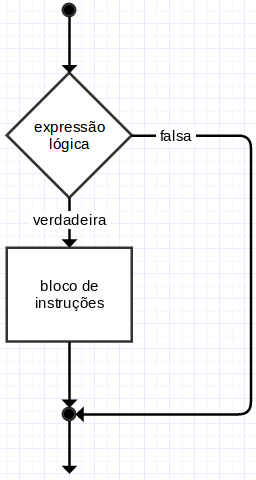
\includegraphics[height=6.0cm]{imagens/condicional_if.png}
							\end{column}
				\end{columns}

		\begin{itemize}
			\item Os espaços \espaco representam aqui a indentação:
			\item As chaves \{\} definem o bloco de instruções que será executado caso a expressão lógica seja \textbf{verdadeira}
		\end{itemize}
	\end{frame}
	
	\begin{frame} 
	Por exemplo:
			\lstinputlisting{exemploIf.c}
	\end{frame}

	\begin{frame}
	\begin{alertblock}{\ding{46} Exercício em sala}
	Escreva um programa que leia do usuário um número \textbf{real} a e um \textbf{inteiro} b. Em seguida, se o número b for diferente de zero, escreva na tela o resultado da divisão $\frac{a}{b}$.

	\end{alertblock}
	\end{frame}

	\begin{frame}
	\begin{alertblock}{\ding{46} Exercício em sala}
	Escreva um programa em C que leia do usuário 3 números reais (a, b e c) e escreva na tela as raízes da equação de acordo com a quantidade de raízes reais.
	$$ ax^2 + bx + c = 0$$

	Teste o seu programa com as seguintes entradas:
	\begin{itemize}
	\item a = 2, b = 6 e c = 3
	\item a = 1, b = 4 e c = 4
	\item a = 1, b = 1 e c = 1
	\end{itemize}
	\end{alertblock}
	\end{frame}


	%%%%%%%%%%%%%%%%%%%%%%%%%%%%%%%% IF/ELSE
	\section{Condicional if/else}
	\begin{frame}[c]
		\begin{center}
			\structure{\large Estrutura de Seleção \textbf{if/else}}
		\end{center}
	\end{frame} 
	\begin{frame} 

				\begin{columns}[t]
					\begin{column}[T]{.4\textwidth}
						if (\exp[expressão lógica]) \{\\
						\espaco \exp[instrução 1]\\
						\espaco \exp[instrução 2]\\
						\espaco \exp[...]\\
						\espaco \exp[instrução n]\\
						\} else \{\\
						\espaco \exp[instrução 1]\\
						\espaco \exp[instrução 2]\\
						\espaco \exp[...]\\
						\espaco \exp[instrução n]\\
						\}
					\end{column}
							\begin{column}[T]{.4\textwidth}
								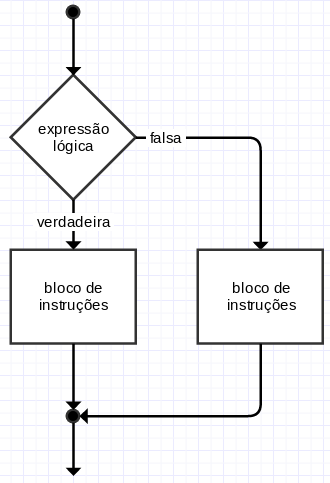
\includegraphics[height=5.5cm]{imagens/condicional_ifelse.png}
							\end{column}
				\end{columns}

		\begin{itemize}
			\item O par de chaves do \textdf{if} definem o bloco de instruções que será executado caso a expressão lógica seja \textbf{verdadeira}
			\item O par de chaves do \textdf{else} definem o bloco de instruções que será executado caso a expressão lógica seja \textbf{falsa}
		\end{itemize}
	\end{frame}

	\begin{frame} 
	Por exemplo:
			\lstinputlisting{exemploIfElse.c}
	\end{frame}

	\begin{frame}
	\begin{alertblock}{\ding{46} Exercício em sala}
	Escreva um programa em C que leia dois números inteiros \textbf{a} e \textbf{b} (assuma que o usuário digita $a > 0$ e $b > 0$). Em seguida deve escrever na tela \texto{Um dos números divide o outro} caso um dos números divida o outro ou \texto{Nenhum dos números divide o outro} caso nenhum dos números divida o outro.
	\end{alertblock}
	\end{frame}

%%%%%%%%%%%%%%%%% CONDICIONAIS ANINHADOS %%%%%%%%%%%%%%%%%
	\section{Condicionais aninhados}
	\begin{frame}[c]
		\begin{center}
			\structure{\large \insertsection}
		\end{center}
	\end{frame} 
	\begin{frame} 
		O bloco de instruções pode incluir outros condicionais (\textdf{condicionais aninhados})!
			\lstinputlisting{codigo5.c}
	\end{frame}

	\begin{frame} 
		Utilizando if/else no problema da aprovação do aluno:
			\lstinputlisting{codigo9.c}
	\end{frame}

	\begin{frame}
	\begin{alertblock}{\ding{46} Exercício em sala} 
		Escreva um programa que leia o número de gols de um time de futebol A e o número de gols de um time B no tempo normal em uma partida de futebol. Se houver um vencedor, o programa deve informar qual foi o time. Mas, se houver empate, o programa deverá solicitar o número de gols de cada uma das equipes nos pênaltis e, em seguida, qual foi o time vencedor (não há mais possibilidade de empates).

		Exemplo 1:\\
		\colorbox{gray!15}{
			\begin{varwidth}{10cm}
				Digite o numero de gols do time A: \textbf{3}\\
				Digite o numero de gols do time B: \textbf{2}\\
				Vencedor: time A
			\end{varwidth}
		}\\

		Exemplo 2:\\
		\colorbox{gray!15}{
			\begin{varwidth}{10cm}
				Digite o numero de gols do time A: \textbf{3}\\
				Digite o numero de gols do time B: \textbf{3}\\
				Digite o numero de gols do time A nos penaltis: \textbf{3}\\
				Digite o numero de gols do time B nos penaltis: \textbf{5}\\
				Vencedor: time B
			\end{varwidth}
		}\\

	\end{alertblock}
	\end{frame}


\end{document}